%% This is file `prletters-template.tex',
%% 
%% Copyright 2013 Elsevier Ltd
%% 
%% This file is part of the 'Elsarticle Bundle'.
%% ---------------------------------------------
%% 
%% It may be distributed under the conditions of the LaTeX Project Public
%% License, either version 1.2 of this license or (at your option) any
%% later version.  The latest version of this license is in
%%    http://www.latex-project.org/lppl.txt
%% and version 1.2 or later is part of all distributions of LaTeX
%% version 1999/12/01 or later.
%% 
%% The list of all files belonging to the 'Elsarticle Bundle' is
%% given in the file `manifest.txt'.
%% 
%% Template article for Elsevier's document class `elsarticle'
%% with harvard style bibliographic references
%%
%% $Id: prletters-template-with-authorship.tex 69 2013-07-15 10:15:25Z rishi $
%%
%% This template has no review option
%% 
%% Use the options `twocolumn,final' to obtain the final layout
\documentclass[times,twocolumn,final,authoryear]{elsarticle}

%% Stylefile to load PR Letters template
\usepackage{prletters}
\usepackage{framed,multirow}

%% The amssymb package provides various useful mathematical symbols
\usepackage{amssymb}
\usepackage{latexsym}

% Following three lines are needed for this document.
% If you are not loading colors or url, then these are
% not required.
\usepackage{url}
\usepackage{xcolor}
\definecolor{newcolor}{rgb}{.8,.349,.1}

%%%%%%%%%%%%%%%
% jdelatorre added header
\usepackage{tikz}
\usepackage{blindtext, graphicx}
\usepackage{smartdiagram}
\newcommand{\degree}{\ensuremath{^{\circ}}\xspace} % adds degree sign 
\usepackage[utf8]{inputenc}
\usepackage[T1]{fontenc} % adds capability to < sign
\usepackage{mathptmx}
\usepackage{amsmath}

% forced line break inside a tabular cell
\newcommand{\specialcell}[2][c]{%
	\begin{tabular}[#1]{@{}c@{}}#2\end{tabular}}

% use it for example as \specialcell[t]{Foo\\bar} or \specialcell{Foo\\bar}
%%%%%%%%%%%%%%%

\journal{Pattern Recognition Letters}

\begin{document}

\thispagestyle{empty}
                                                             
\begin{table*}[!th]

\begin{minipage}{.9\textwidth}
\baselineskip12pt
\ifpreprint
  \vspace*{1pc}
\else
  \vspace*{-6pc}
\fi

\noindent {\LARGE\itshape Pattern Recognition Letters}
\vskip6pt

\noindent {\Large\bfseries Authorship Confirmation}

\vskip1pc


{\bf Please save a copy of this file, complete and upload as the 
``Confirmation of Authorship'' file.}

\vskip1pc

As corresponding author 
I, \underline{Jordi de la Torre}, 
hereby confirm on behalf of all authors that:

\vskip1pc

\begin{enumerate}
\itemsep=3pt
\item This manuscript, or a large part of it, \underline {has not been
published,  was not, and is not being submitted to} any other journal. 

\item If \underline {presented} at or \underline {submitted} to or
\underline  {published }at a conference(s), the conference(s) is (are)
identified and  substantial \underline {justification for
re-publication} is presented  below. A \underline {copy of
conference paper(s) }is(are) uploaded with the  manuscript.

\item If the manuscript appears as a preprint anywhere on the web, e.g.
arXiv,  etc., it is identified below. The \underline {preprint should
include a  statement that the paper is under consideration at Pattern
Recognition  Letters}.

\item All text and graphics, except for those marked with sources, are
\underline  {original works} of the authors, and all necessary
permissions for  publication were secured prior to submission of the
manuscript.

\item All authors each made a significant contribution to the research
reported  and have \underline {read} and \underline {approved} the
submitted  manuscript. 
\end{enumerate}

Signature\underline{\hphantom{\hspace*{7cm}}} Date\underline{\hphantom{\hspace*{4cm}}} 
\vskip1pc

\rule{\textwidth}{2pt}
\vskip1pc

{\bf List any pre-prints:}
\vskip5pc


\rule{\textwidth}{2pt}
\vskip1pc

{\bf Relevant Conference publication(s) (submitted, accepted, or
published):}
\vskip5pc



{\bf Justification for re-publication:}

\end{minipage}
\end{table*}

\clearpage
\thispagestyle{empty}
\ifpreprint
  \vspace*{-1pc}
\fi

\begin{table*}[!th]
\ifpreprint\else\vspace*{-5pc}\fi

\section*{Graphical Abstract (Optional)}
To create your abstract, please type over the instructions in the
template box below.  Fonts or abstract dimensions should not be changed
or altered. 

\vskip1pc
\fbox{
\begin{tabular}{p{.4\textwidth}p{.5\textwidth}}
\bf Type the title of your article here  \\
Author's names here \\[1pc]

\includegraphics[width=.3\textwidth]{top-elslogo-fm1.pdf}
& 
This is the dummy text for graphical abstract.
This is the dummy text for graphical abstract.
This is the dummy text for graphical abstract.
This is the dummy text for graphical abstract.
This is the dummy text for graphical abstract.
This is the dummy text for graphical abstract.
This is the dummy text for graphical abstract.
This is the dummy text for graphical abstract.
This is the dummy text for graphical abstract.
This is the dummy text for graphical abstract.
This is the dummy text for graphical abstract.
This is the dummy text for graphical abstract.
This is the dummy text for graphical abstract.
This is the dummy text for graphical abstract.
This is the dummy text for graphical abstract.
This is the dummy text for graphical abstract.
This is the dummy text for graphical abstract.
This is the dummy text for graphical abstract.
This is the dummy text for graphical abstract.
This is the dummy text for graphical abstract.
This is the dummy text for graphical abstract.
This is the dummy text for graphical abstract.
This is the dummy text for graphical abstract.
This is the dummy text for graphical abstract.
%}\\
\end{tabular}
}

\end{table*}

\clearpage
\thispagestyle{empty}

\ifpreprint
  \vspace*{-1pc}
\else
%  \vspace*{-6pc}
\fi

\begin{table*}[!t]
\ifpreprint\else\vspace*{-15pc}\fi

\section*{Research Highlights (Required)}

To create your highlights, please type the highlights against each
\verb+\item+ command. 

\vskip1pc

\fboxsep=6pt
\fbox{
\begin{minipage}{.95\textwidth}
It should be short collection of bullet points that convey the core
findings of the article. It should  include 3 to 5 bullet points
(maximum 85 characters, including spaces, per bullet point.)  
\vskip1pc
\begin{itemize}

 \item Formulation of a new loss function for the optimization of multi-class classification of ordinal data based on the weighted kappa index to be used in supervised deep learning architectures.

 \item Comparison of the performance achieved between the new loss and the standard logarithmic loss function using a diabetic retinopathy image classification problem.

 \item Check the stability of the new loss function using different input and batch sizes.

 \item

 \item

\end{itemize}
\vskip1pc
\end{minipage}
}

\end{table*}

\clearpage


\ifpreprint
  \setcounter{page}{1}
\else
  \setcounter{page}{1}
\fi

\begin{frontmatter}

\title{Weighted kappa loss function for multi-class classification of ordinal data in deep learning}

\author[1]{Jordi \snm{de la Torre}} 
\author[1]{Domenec \snm{Puig}}
\author[1]{Aida \snm{Valls}\corref{cor1}}

\cortext[cor1]{Corresponding author: 
	Tel.: +34-977-559-708;  
	fax: +34-977-559-699;}
\ead{aida.valls@urv.cat}

\address[1]{Departament d'Enginyeria Inform\`{a}tica i Matem\`{a}tiques\\ Universitat Rovira i Virgili \\ Avinguda Pa\"{i}sos Catalans, 26 \\ ES-43007 Tarragona}

\received{30 Jan 2017}
\finalform{30 Jan 2017}
\accepted{30 Jan 2017}
\availableonline{30 Jan 2017}
\communicated{S. Sarkar}


\begin{abstract}

Weighted Kappa is a index of reference used in many diagnosis systems to compare the agreement between different raters. This index can be also used to compare the goodness of a machine-learning based classification method against the results gotten from a consensus expert group. On the other hand, deep learning has achieved in the last years a great importance as a machine learning method for designing classification algorithms also for medical diagnosis. In this paper we explore the direct use of a Weighted Kappa loss function for the optimization of classification ratings, where one ore more underlying causes induce some pr-established ordering of the classes to predict. We show that for the case of diabetic retinopathy image classification, better results can be obtained from the direct optimization of Kappa over the results obtained from the usage of a multi-class logarithmic loss function.

\end{abstract}

\begin{keyword}
\MSC 62H35\sep 82C32\sep 62M45
\KWD deep learning\sep convolutional neural networks\sep supervised learning\sep computer vision\sep diabetic retinopathy\sep cohen's kappa\sep loss function\sep ordinal data\sep weighted kappa\sep ordinal regression

%% MSC codes here, in the form: \MSC code \sep code
%% or \MSC[2008] code \sep code (2000 is the default)
\end{keyword}

\end{frontmatter}

%\linenumbers

\section{Introduction}

Deep Learning methods have been used extensively in the last years for many automatic classification tasks. The scheme used for images, is based on extracting the important features with a set of convolutional layers and after that make a final classification with them using a set of fully connected layers. A last soft-max output layer gives as a result the predicted output probabilities of the set of classes the model. During training the model parameters are changed using a gradient based optimization algorithm, minimizing a predefined loss function. For multi-class classification the standardized loss function to use is the logarithmic loss (log-loss).

On the other hand, weighted kappa index is used in medical diagnosis systems for measuring the level of agreement between raters \citep{hripcsak2002measuring}, in the applications where some underlying factors present on images or data, need to be interpreted in order to infer from them a diagnose. In this interpretation normally is present some level of subjectivity that make sometimes the conclusions of different experts to differ. Weighted kappa ($\kappa$) is able to measure the level of discrepancy of a set of diagnosis made by different raters over the same population \citep{viera2005understanding}. Depending on the value of the index, the strength of agreement between the raters can be evaluated (see table \ref{tab:kappa_int}). 

Examples of the usage of the $\kappa$ index for measuring inter-rater agreement are the measure of reliability in ultrasound scans interpretation \citep{hintz2007interobserver}, evaluation of expert agreement in diagnosis of glaucoma \citep{varma1992expert}, evaluation of reliability of radiographic assessment \citep{gunther1999reliability}, inter-observer agreement evaluation in diabetic retinopathy detection \citep{patra2009interobserver}, between many others. $\kappa$ takes into account the pr-established ordering of the classes and penalizes the erroneous predictions in function of the distance. In that way, a failure in a prediction that is close to the real category is considered better than a prediction that is farthest. 

This index can be used also to measure the goodness of the prediction given by a machine learning method. The values of the prediction can be compared against the correct values reported by a human experts consensus group. In that way, the index compares the values predicted by the model with the considered "true value" coming from the consensus of a human experts group.


\begin{table}
	\caption{\label{tab:kappa_int}Table interpretation of Weighted Kappa, after Landis \& Koch (1977)}	
	\centering
	\begin{tabular}{llr}
		\hline
		QWK    & Strength of agreement \\
		\hline
		<0.20 		& Poor \\
		0.21-0.40 	& Fair \\
		0.41-0.60 	& Moderate \\
		0.61-0.80 	& Good \\
		0.81-1.00 	& Very good \\
		\hline
	\end{tabular}
\end{table}

In this paper, we study the direct optimization of $\kappa$, using it not only as a evaluation function but also as loss function. We use a diabetic retinopathy image classification problem to check its stability and to compare the performance of the results obtained from the use of the standard logarithmic loss against the results obtained from the optimization of $\kappa$.

The study is organized as follows: we present the background of this work showing the standardized loss function used for classification, next we propose the new cost function for multi-class classification of ordinal data (ordinal regression) with all the mathematical equations required for the optimization, we define the experiments, the results obtained and finally present the conclusions.

\section{Deep learning method}

Supervised deep learning techniques are used extensively for many automatic classification tasks. In the case of images, most of the state of the art methods are based on the use of deep convolutional neural networks (CNN). These techniques are focused on learning multiple levels of representation and abstraction that help to make sense of the hidden information in data such as images. In this way, having a complete set of correctly classified images and without any a priori understanding of the features, the system is able to learn the properties of the image that minimize a defined cost function that is direct or indirectly related with the classification score index to optimize (see fig. \ref{fig:classification}). 

\begin{figure}[!h]
	\label{fig:classification}
	\centering
	\smartdiagramset{back arrow disabled=true}
	\resizebox{.9\linewidth}{!}{\smartdiagram[flow diagram:horizontal]{Image Input, Feature Extraction Layers, Classification Layers, Class Probability, Cost\\Function}}
	\caption{High level description of a deep learning image classification scheme}
\end{figure}

For image classification a convolutional neural network is used for making the automatic feature extraction followed by a one or more classification layers (normally fully connected layers) and a final output layer formed by as many outputs as classes to predict. It is usual to have in such an output layer a soft-max function that represents the output probability of every class to predict. Normally, the chosen class is the one with the highest value of probability in the output layer. This neural network architecture has a set of parameters on every layer that have to be optimized to achieve the most accurate prediction of the data. This is done by optimizing a function of the output variables, called loss function. This function depends on the output probabilities given by the model and is defined in a way that minimizing it maximizes the probability of the correct class. If the defined function is differentiable with respect to the output variables then is possible to apply a gradient descent based algorithm to optimize the function. In every optimization step the classification derivative of the loss function is calculated and back-propagated through the network. The parameters are updated accordingly to the optimization algorithm in order to reduce de discrepancy between the output of the model and the true value given by the known data.

Multi-class classification is addressed mainly by the optimization of the logarithmic loss function (see eq. \ref{eq:logloss}). This function is very easy to optimize using gradient descent methods due to the simplicity of its derivatives, its numerical stability and experimental tested validity \citep{Goodfellow-et-al-2016}. Additionally, the logarithmic loss has a very robust probabilistic foundation: minimizing it is the same as minimizing the logarithmic likelihood, that is equivalent to do a maximum likelihood estimation (MLE) or equivalently, to find the maximum a posteriori probability (MAP), given a uniform prior \citep{Murphy:2012:MLP:2380985}. This function does not encode any prior information about the classes and this fact make this function a general purpose function that performs well in many applications. 

\begin{equation}
\begin{aligned}
\label{eq:logloss}
&\mathcal{L} = \frac{1}{N} \sum_{i=1}^N \sum_{c=1}^C t_i \log{y_i^{(c)}}
\end{aligned}
\end{equation}

Where:
\begin{itemize}
	\item[] N: is the number of samples
	\item[] $t_i$: is 1 for the correct class of sample i and 0 elsewhere
	\item[] C: is the number of classes
\end{itemize}

On the other hand, there are applications where we have a priori information about some property of the classes. For example, in the case of ordinal regression, the different categories are sorted in a predefined way that intends to classify into categories the gradation of some intrinsic information. When the log-loss is applied for the classification in this problems, it has to learn from the data such a pr-established ordering. In those cases, its general capability can become disadvantage. A loss that encodes such a prior information about the intrinsic property of the classes can perform better or faster due to the fact that does not require to learn it from the available data. 

\section{QWK Loss Function}

In this section we present our contribution to the optimization of CNN using weighted kappa. Weighted Kappa (see eq. \ref{eq:kappa}) is normally used as an index to measure the inter-rating agreement between a set of different classes where these categories have a predefined ordering in such a way that the property that we want to categorize is a high level abstraction of the level of some sort of intrinsic information that we want to extract from the categorization. 

\begin{equation}
\label{eq:kappa}
\begin{aligned}
&\kappa = 1 - \frac{ \sum_{i,j} \omega_{i,j} O_{i,j} }
{\sum_{i,j} \omega_{i,j} E_{i,j}}\\
\end{aligned}
\end{equation}

Where:
\begin{itemize}
	\item[] C: is the number of classes
    \item[] $i, j \in \{ 1, 2, ..., C\}$
	\item[] $O_{i,j}$: the number of observations that received a rating of i by observer A (prediction) and a rating of j by observer B ("true value").
	\item[] $E_{i,j}$: outer product between each rater's histogram vector of ratings (prediction and "true value"), normalized such that E and O have the same sum.
	\item[] $\omega_{i,j}$: weight penalization for every pair of classes. Frequently used $\omega_{i,j} = \frac{(i-j)^n}{(C - 1)^n}$. For linear penalization $n = 1$. For quadratic penalization (more commonly used and the studied in this paper): $n = 2$.
\end{itemize}

This index establishes a penalization when there is a discrepancy between the raters that depends on the distance between both predictions. In the case of the Quadratic Weighted Kappa (QWK) the penalization of the discrepancy grows quadratically with the distance between the two ratings. If the predicted classes of both raters is the same, we say the there is an \emph{absolute} concordance between both raters and no penalization is applied. When the predicted classes are different, we say that the there is \emph{relative} concordance between both raters and there is a penalization in the calculation of the inter-rating index that is proportional, in the case of QWK, to the square of the distance between both predictions. This discrepancies are calculated for all the N items of the k mutually exclusive categories and summed over the N items. The penalizing term is normalized dividing their value by the expected  discrepancy, obtaining as a result a value between -1 and 1. A value of 1 of the index would indicate a perfect agreement between both raters, -1 a perfect symmetric disagreement between the classes and 0 a random evaluation method. 

\subsection{Mathematical foundation}

The optimization problem that we want to solve in order to maximize the probabilities of the true classes of our model using the $\kappa$ function is presented in equation \ref{eq:optim}

\begin{equation}
\label{eq:optim}
\begin{aligned}
& \underset{x}{\text{maximize}}
& & \kappa = 1 - \frac{ \sum_{i,j} \omega_{i,j} O_{i,j} }
{\sum_{i,j} \omega_{i,j} E_{i,j}} & & \kappa \in [-1,1]\\
\end{aligned}
\end{equation}

This problem can be redefined in the form of equation \ref{eq:optim-redef} in order change the maximization problem to a minimization one. Loss function are defined as minimization problems, that's why we redefine the problem to solve it as a minimization one. Taking the log we change the output range and increment the numerical stability of the problem.

\begin{equation}
\label{eq:optim-redef}
\begin{aligned}
& \underset{x}{\text{minimize}}
& & \mathcal{L} = \log{\left( 1 - \kappa \right)}  & & \mathcal{L} \in \left(-\infty,\log{2}\right]
\end{aligned}
\end{equation}


As we want to use the index as a optimization function, we have to take into account that our model will not report a predicted class as an output but a probability for every class. That's why the observed values given by our model will not be integer values but real ones. In eq. \ref{eq:num} we show the expression of the numerator of the $\kappa$ function for taking into account the probabilities of every prediction. In eq. \ref{eq:den} we also show the redefinition of the denominator of the same index in order to take into account the probabilities given by the model. 

\begin{equation}
\label{eq:num}
 \mathcal{N} = \sum_{i,j} \omega_{i,j} O_{i,j} = \sum_{k=1}^N \sum_{c=1}^C \omega_{t_k,c} P_c(X_k) 
\end{equation}
\begin{equation}
\label{eq:den}
\mathcal{D} = \sum_{i,j} \omega_{i,j} E_{i,j} = \sum_{i=1}^C \hat{N_i} \sum_{j=1}^C \left( \omega_{i,j} \sum_{k=1}^N P_j(X_k)\right)
\end{equation}

Where:
\begin{itemize}
	\item[] $X_k$: input data of sample k
	\item[] $E_{i,j} = \frac{N_i \sum_{k=1}^N P_j(X_k)}{N} = \hat{N_i} \sum_{k=1}^N P_j(X_k)$
	\item[] N: number of samples
	\item[] $N_i$: number of samples of class i
	\item[] $\hat{N_i}$ = $\frac{N_i}{N}$	
	\item[] $t_k$: correct class number for sample k
	\item[] $P_c(X_k)$: probability that sample k is of class C given that the true class in $t_k$
\end{itemize}

\subsection{Partial derivatives of the QWK loss function}

For solving this optimization problem using any gradient descent based algorithm, we need to derive the partial derivatives of the loss function with respect to the output variables of the network. 

For the case minimizing the loss function $\mathcal{L} = \log{ \frac{\mathcal{N}}{\mathcal{D}}}$, the derivative takes the next form:

\begin{equation}
\frac{\partial \mathcal{L}}{\partial y_m} = \frac{1}{\mathcal{N}}\frac{\partial \mathcal{N}}{\partial y_m} - \frac{1}{\mathcal{D}}
\frac{\partial{\mathcal{D}}}{\partial y_m}
\end{equation}

And $\frac{\partial \mathcal{N}}{\partial y_m}$ and $\frac{\partial{\mathcal{D}}}{\partial y_m}$ can be calculated with the next expressions:

\begin{equation}
\frac{\partial \mathcal{N}}{\partial y_m(X_k)} = \omega_{t_k m}
\end{equation}

\begin{equation}
\frac{\partial \mathcal{D}}{\partial y_m(X_k)} = \sum_{i=1}^{C} \hat{N_i} \omega_{i,m}
\end{equation}

Where: 
\begin{itemize}
\item[] $m \in \{1, 2, ..., C\}$
\end{itemize}

That in its array form can be rewritten as:


\begin{equation}
\begin{aligned}
\frac{\partial \mathcal{N}}{\partial y_m} =
\begin{pmatrix} 
\omega_{t_1, 1}     & \omega_{t_1, 2}     & ...     & ... & \omega_{t_1, C}\\ 
\omega_{t_2, 1}     & \omega_{t_2, 2}     & ...     & ... & \omega_{t_2, C}\\ 
...					& ...		          & ...     & ... & ...\\
\omega_{t_N, 1}     & \omega_{t_N, 2}     & ...     & ... & \omega_{t_N, C}\\  
\end{pmatrix}
\end{aligned}
\end{equation}

\begin{equation}
\begin{aligned}
\frac{\partial \mathcal{D}}{\partial y_m} =
\begin{pmatrix} 
\sum_{i=1}^C \hat{N_i} \omega_{1,i} & ...  & ...     & ... & \sum_{i=1}^C \hat{N_i} \omega_{C,i}\\
\sum_{i=1}^C \hat{N_i} \omega_{1,i} & ...  & ...     & ... & \sum_{i=1}^C \hat{N_i} \omega_{C,i}\\
... & ::: & ... & ... & ...\\
\sum_{i=1}^C \hat{N_i} \omega_{1,i} & ...  & ...     & ... & \sum_{i=1}^C \hat{N_i} \omega_{C,i}\\ 
\end{pmatrix}
\end{aligned}
\end{equation}

With the definition of the loss function and its derivatives we have all the equations required to apply to our model any first order optimization algorithm to fit the data. 

\section{Experiments}

The finality of the experiments of this paper is to test the proposed optimization loss function against a real example. We have chosen a diabetic retinopathy image classification task. Here below, we define the problem, describe the data and finally define the procedure the we have used to test the performance of the new loss.

\subsection{Classification Problem Definition}

Diabetic Retinopathy (DR) is a leading disabling chronic disease  and  one of the main causes of blindness and visual impairment in developed countries for diabetic patients. Studies reported that 90\% of the cases can be prevented through early detection and treatment \cite{torrents15}. Eye screening through retinal images is used by physicians to detect the lesions related with this disease. Due to the increasing number of diabetic people, the amount of images to be manually analyzed is becoming unaffordable. Moreover, training new personnel for this type of image-based diagnosis is long, because it requires to acquire expertise by daily practice. 

In 2003 the medical community established a standardized classification based on four severity stages \cite{diaclass} determined by the type and number of lesions (as micro-aneurysms, hemorrhages and exudates): class 0 referring to no apparent retinopathy, class 1 as a Mild Non-Proliferative Diabetic Retinopathy (NPDR), class 2 as Moderate NPDR, class 3 as a Severe NPDR and class 4 as a Proliferative DR. 

The problem consist on optimize a deep convolutional neural network to maximize the classification rates over a test set of never seen before images. The generalization capability will be scored against the quadratic weighted kappa over the test set.

\subsection{Data}

The dataset used in this work consists of two independent high resolution image sets (train and test). For every patient right and left eye images are reported. All the images are classified by ophthalmologists according to the standard severity scale presented before \cite{diaclass}. The images are taken in variable conditions: by different cameras, illumination conditions and resolutions. 

The training set contains a total of 35.126 images; 25.810 of class 0, 2.443 of class 1, 5.292 of class 3, 873 of class 3 and 708 of class 4. The test set contains a total of 53.576 images; 39.533 of class 0, 3.762 of class 1, 7.861 of class 2, 1.214 of class 3 and 1.206 of class 4. Notice that it is highly imbalanced.

\subsection{The models}

In this section we define the models that we have used to compare the performance of the to losses. Four different models have been used, one for every different image size. The idea was to first design smaller models based on restricted image sizes in order to have a small training time that could allow to test the maximum amount of experiments. This big set of previous experiments would allow to restrict the hyper-parameter space. Bigger models, more slower to train, would then be trained with the better selection of hyper-parameters.

All the models follow the scheme defined in fig. \ref{fig:classification}. The feature extraction layers use all 3x3 convolutions with padding of 1 and stride 1, followed by a batch normalization\citep{batch-norm} and a ReLU activation function \citep{Dahl2013}. Every two feature layers a 2x2 max-pooling layer of stride 2 is applied for dimensionality reduction. The number of feature layers vary depending on the image size. All the models use an unique classification layer followed by the final output soft-max layer. The number of layers and the total number of parameters of each model are summarized in table \ref{tab:models}.

The model used for the 128x128 image case has 1.16 million of parameters, 10 feature lavers of 32/32, 64/64, 128/128, 128/128 filters in every convolution (/ separate the filters for every map size, the commas indicate a 2x2 max-pooling operation) and a 4x4 convolution classification layer of 128 filters. The model used for the 256x256 image case has 1.44 million of parameters, 12 feature lavers of 32/32, 64/64, 128/128, 128/128, 128/128 filters in every convolution and a 4x4 convolution classification layer of 128 filters. The model used for the 384x384 image case has 1.77 million of parameters, 12 feature lavers of 32/32, 64/64, 128/128, 128/128, 128/128 filters in every convolution and a 6x6 convolution as a classification layer of 128 filters. Finally, the model used for the 512x512 image case has 11.3 million of parameters, 12 feature lavers of 16/16, 32/32, 64/64, 128/128, 256/256, 512/512 filters in every convolution, a 5x5 convolution as classification layer of 512 filters, followed by a 4x4 average pooling and a dropout layer (ratio = 0.3).

\subsection{Procedure}

We define a set of experiments to compare the performance of the model when its parameters are optimized using the log-loss and the QWK loss. We want to check if the encoding of the ordering of the classes helps in the improvement of the generalization results. In order to make the comparison possible, every model will be optimized with both functions. The final generalization capability of the same model optimized with both functions will be compared. 

As deep learning is a computer intensive task, the experiments have been done using models of different input resolution images: 128x128, 256x256, 384x384 and 512x512. The lower time required to train low resolution images allow to run more experiments and serve to not only make a first validation of the new cost function but also to make a first hyper-parameters selection that can serve later on to validate the new cost function against higher resolution images using less time consuming experiments.

The original training set is split in two random subsets: one with 90\% of the data and other with 10\%. The last one is used as a validation set for hyper-parameter selection. The value of QWK is calculated every epoch either for the training or the validation set. 

Notice that the image set is highly imbalanced. In order facilitate the training the training set is artificially equalized using data augmentation techniques based on 0-360\degree random rotation, X and Y mirroring and contrast and brightness random sampling.

A random initialization based in the Kaiming\&He approach \citep{kaiming} is used for all the networks. All models are optimized using Adam \citep{DBLP:journals/corr/KingmaB14} over batches. We study different learning rates in order to find the optimal one for each loss function. We use a batch-based optimization algorithm. QWK loss function uses a normalization term that normalizes over the sample set. Presumably this loss function has to be more sensible to small batches that the logarithmic loss due to this normalization term, that's why different batch sizes are tested. For every batch, the images are chosen randomly from the training set, with repetition. Data augmentation techniques are applied to augment the diversity of the classes (random rotations and brightness and contrast modifications). The epoch size is set to maintain fixed the total number of images per epoch to 100.000. This value is approximately the number of images required to sample to ensure that all of them has been selected every epoch. Also, using different batch sizes, the number of updates per epoch of the parameters of the neural network change. In the case of small batch sizes the number of updates per epoch is greater than the case of big batch sizes. Studying different batch sizes we would also explore different number of parameter updates. All the tests were run for 100 epochs.

\section{Results}

Table \ref{tab:qwk_cv} shows the experiments using both losses with different learning rates and batch sizes. QWK score is calculated over the validation set for comparison between the results obtained from the direct optimization of the function and the standardized indirect method of using the log-loss function. 

In figure \ref{fig:best} we show a graphical representation of the maximum value of QWK on the test set for the different tested configurations. We can see that directly optimizing QWK gives consistently better results than optimizing log-loss. Only in the case of very small batch sizes (in this case, BS = 5) log-loss performs better than QWK. This is probably due to the fact that QWK uses a normalization term in the denominator that with not big enough batch sizes could cause instabilities in the gradient that affect the performance. In any case, even in those cases the results obtained with the log-loss are worse that those achieved using the best QWK configuration.

The optimal batch size for solving this diabetic retinopathy classification is of 5 in the case of using the log-loss and 15 in the case of the QWK-loss. For greater values of this hyper-parameter, the increase of precision in the calculation of the gradient does not gives any advantage in the optimization. In the case of the log-loss a lower precision in the calculation of the gradient works better. This fact could probably is due to the fact that this imprecision in the calculation increases the stochasticity of the prediction and due to the fact that we are not optimizing directly the metrics index this make possible to explore adjacent zones that could work better for improving the metrics index that the ones that specifically improve the log-loss. Additionally, although smaller batch sizes give worse approximations of the gradient, the number of updates per epoch of the parameters of the model is greater. This seems to be an advantage in this case.



\begin{figure}[!htb]
	\centering
	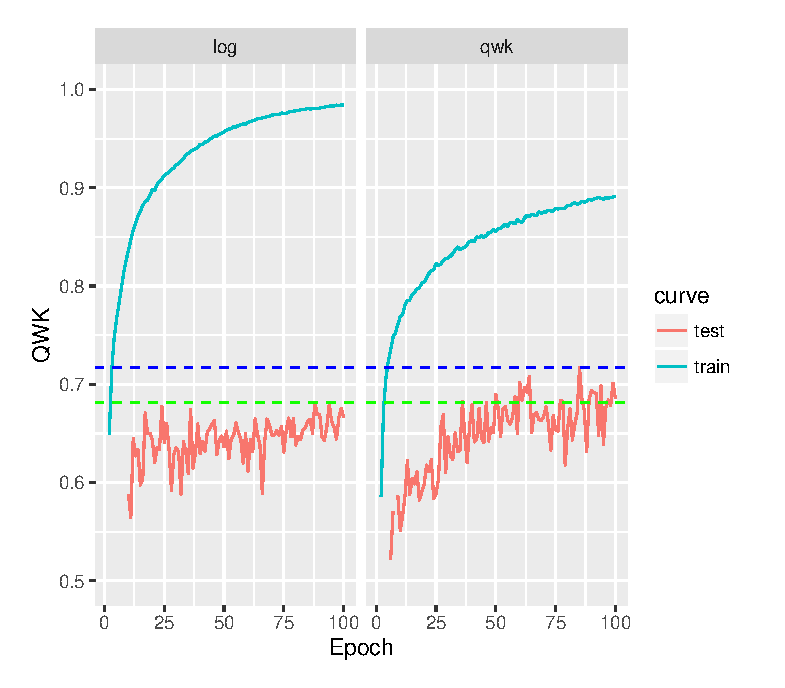
\includegraphics[scale=.70]{training-curves.eps}
	\caption{Evolution of QWK values during training for logarithmic and QWK loss functions (512x512 input image case)}
	\label{fig:training-curves}
\end{figure}

\begin{figure}[!htb]
	\centering
	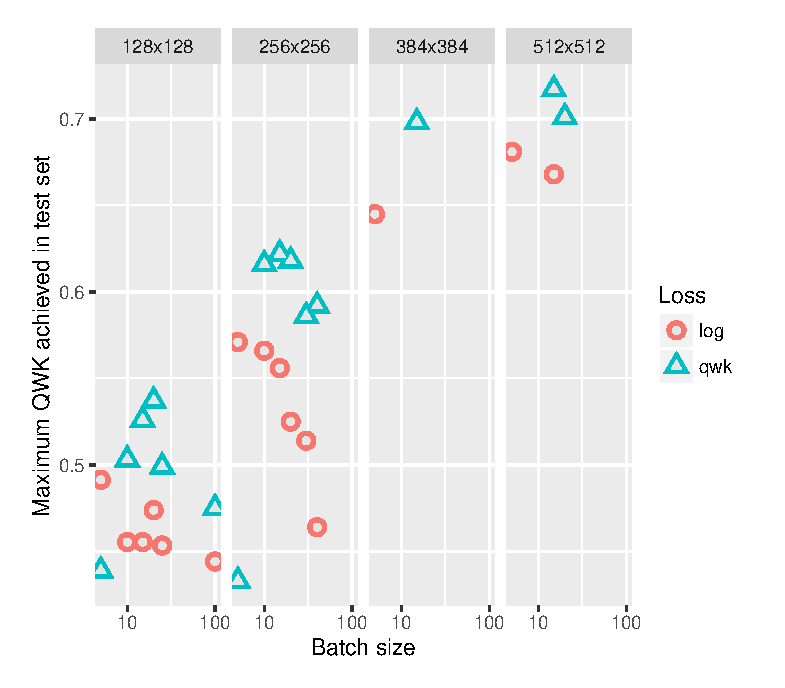
\includegraphics[scale=.70]{best.eps}
	\caption{Best classification results achieved over test set for each loss function}
	\label{fig:best}
\end{figure}

\begin{table}[h!]
	\centering
	\caption{Results achieved in different experiments}
	\label{tab:qwk_cv}
	\resizebox{\columnwidth}{!}{ 
	\begin{tabular}{c|c|c|c|c|c|c|c|c}
		Input & BS & Loss & LR	& $\kappa_{train} 10^3$ & $\kappa_{test} 10^3$ & Gap & Epoch & Updates $10^{-3}$\\	
		\hline
		\multirow{32}{*}{128} & \multirow{6}{*}{5} & \multirow{3}{*}{log} & $10^{-5}$ & 771 & 418 & 353 & 78 & 1560\\
		& & & $10^{-4}$ & 851 & \textbf{491} & 360 & 73 & 1460\\
		& & & $10^{-3}$ & 676 & 418 & 258 & 29 & 580\\\cline{3-9}
		& & \multirow{3}{*}{qwk} & $5 \times 10^{-5}$ & 545 & 402 & 143 & 50 & 1000\\
		& & & $10^{-5}$ & 646 & 439 & 207 & 70 & 1400\\
		& & & $10^{-4}$ & 497 & 326 & 171 & 31 & 620\\\cline{2-9}
		&\multirow{6}{*}{10} & \multirow{3}{*}{log} & $10^{-5}$ & 797 & 397 & 400 & 82 & 820\\
		& & & $10^{-4}$ & 874 & 455 & 419 & 81 & 810\\
		& & & $10^{-3}$ & 514 & 336 & 178 & 57 & 570\\\cline{3-9}
		& & \multirow{3}{*}{qwk} &  $10^{-5}$ & 774 & 476 & 298 & 82 & 820\\
		& & & $10^{-4}$ & 755 & 503 & 252 & 84 & 840\\
		& & & $10^{-3}$ & 596 & 289 & 307 & 95 & 950\\\cline{2-9}		
		& \multirow{6}{*}{15} & \multirow{3}{*}{log} & $10^{-5}$ & 803 & 368 & 435 & 79 & 527\\
		& & & $10^{-4}$ & 899 & 458 & 441 & 95 & 633\\
		& & & $10^{-3}$ & 868 & 447 & 421 & 80 & 533\\\cline{3-9}
		& & \multirow{3}{*}{qwk} & $5\times10^{-5}$ & 715 & 491 & 224 & 77 & 513\\
		& & & $10^{-4}$ & 800 & 526 & 274 & 77 & 513\\
		& & & $5\times10^{-4}$ & 823 & 523 & 300 & 72 & 480\\\cline{2-9}
		& \multirow{2}{*}{20} & log & $10^{-4}$ & 896 & 474 & 422 & 79 & 395\\\cline{3-9}
		& & qwk & $10^{-4}$ & 835 & \textbf{537} & 298 & 93 & 465\\\cline{2-9}
		& \multirow{6}{*}{25} & \multirow{3}{*}{log} & $10^{-5}$ & 821 & 315 & 506 & 96 & 384\\
		& & & $10^{-4}$ & 913 & 453 & 460 & 93 & 372\\
		& & & $10^{-3}$ & 849 & 382 & 467 & 70 & 280\\\cline{3-9}
		& & \multirow{3}{*}{qwk} & $10^{-5}$ & 808 & 423 & 385 & 95 & 380\\
		& & & $10^{-4}$ & 824 & 499 & 325 & 65 & 260\\
		& & & $10^{-3}$ & 655 & 447 & 208 & 80 & 320\\\cline{2-9}
		& \multirow{2}{*}{100} & \multirow{3}{*}{log} & $10^{-4}$ & 929 & 377 & 552 & 98 & 98\\
		& & & $10^{-3}$ & 947 & 444 & 503 & 99 & 99\\
		& & & $10^{-2}$ & 842 & 412 & 430 & 67 & 67\\\cline{3-9}
		& & \multirow{3}{*}{qwk} & $10^{-4}$ & 879 & 450 & 429 & 93 & 93\\
		& & & $10^{-3}$ & 798 & 455 & 343 & 71 & 713\\
		& & & $10^{-2}$ & - & - & - & - & -\\
		\hline	
		\multirow{10}{*}{256} & \multirow{2}{*}{5} & \multirow{1}{*}{log} & $10^{-4}$ & 871 & \textbf{571} & 300 & 52 & 1040\\\cline{3-9}
		& & \multirow{1}{*}{qwk} & $10^{-4}$ & 605 & 433 & 172 & 15 & 300\\\cline{2-9}
		&\multirow{2}{*}{10} & \multirow{1}{*}{log} & $10^{-4}$ & 903 & 566  & 337 & 75 & 750\\\cline{3-9}
		& & \multirow{1}{*}{qwk} & $10^{-4}$ & 832 & 616 & 216 & 70 & 700\\\cline{2-9}		
		& \multirow{2}{*}{15} & \multirow{1}{*}{log} & $10^{-4}$ & 925 & 556 & 369 & 98 & 653\\\cline{3-9}
		& & \multirow{1}{*}{qwk} & $10^{-4}$ & 878 & \textbf{622} & 256 & 93 & 620\\\cline{2-9}
		& \multirow{2}{*}{20} & \multirow{1}{*}{log} & $10^{-4}$ & 923 & 525 & 398 & 97 & 485\\\cline{3-9}
		& & \multirow{1}{*}{qwk} & $10^{-4}$ & 891 & 618 & 273 & 97 & 485 \\\cline{2-9}		
		& \multirow{2}{*}{30} & \multirow{1}{*}{log} & $10^{-4}$ & 925 & 514 & 411 & 93 & 310\\\cline{3-9}
		& & \multirow{1}{*}{qwk} & $10^{-4}$ & 900 & 586 & 314 & 98 & 327\\\cline{2-9}
		& \multirow{2}{*}{40} & \multirow{1}{*}{log} & $10^{-4}$ & 922 & 464 & 458 & 93 & 233\\\cline{3-9}
		& & \multirow{1}{*}{qwk} & $10^{-4}$ & 894 & 592 & 302 & 78 & 195\\\cline{2-9}
		\hline					
		\multirow{2}{*}{384} & \multirow{1}{*}{5} & \multirow{1}{*}{log} & $10^{-4}$ & 863 & \textbf{641} & 222 & 38 & 760\\\cline{2-9}
		& \multirow{1}{*}{15} & \multirow{1}{*}{qwk} & $10^{-4}$ & 889 & \textbf{698} & 191 & 93 & 620 \\\cline{2-9}
		\hline					
		\multirow{4}{*}{512} & \multirow{1}{*}{5} & \multirow{1}{*}{log} & $10^{-4}$ & 980 & \textbf{681} & 299 & 88 & 1760\\\cline{2-9}
		& \multirow{2}{*}{15} & \multirow{1}{*}{log} & $10^{-4}$ & 978 & 668 & 310 &  94 & 626\\\cline{3-9}
		&  & \multirow{1}{*}{qwk} & $10^{-4}$ & 884 & \textbf{717} & 167 & 86 & 573 \\\cline{2-9}
		& \multirow{1}{*}{20} & \multirow{1}{*}{qwk} & $10^{-4}$ & 903 & 701 & 202 & 89 & 445\\\cline{3-9}			
		\hline
	\end{tabular}
}
\end{table}


\begin{table}[h!]
	\centering
	\caption{Results achieved with every tested model optimizing with log-loss and the new qwk-loss}
	\label{tab:models}
	\resizebox{\columnwidth}{!}{ 
		\begin{tabular}{c|c|c|c|c|c|c|c}
			Input & \specialcell{Total\\Layers} & \specialcell[t]{Feature\\Layers} & \specialcell[t]{Classific.\\Layers} &  \specialcell[t]{Params\\$10^{-6}$} & $\kappa_{test}^{qwk}$ & $\kappa_{test}^{log}$ & $\Delta$\\
			\hline
			128x128 & 12 & 10 & 1 & 1.16 & 0.537 & 0.491 & 9.3 \%\\
			256x256 & 14 & 12 & 1 & 1.44 & 0.622 & 0.571 & 8.9 \%\\
			384x384 & 14 & 12 & 1 & 1.77 & 0.698 & 0.663 & 5.3 \%\\
			512x512 & 14 & 12 & 1 & 11.3 & 0.717 & 0.681 & 5.3 \%\\
			\hline
		\end{tabular}
}
\end{table}

\section{Conclusions}
We presented a new loss function for ordinal regression problems based on the optimization of the weighted kappa index. In contrast to the logarithmic loss that uses a uniform prior over the set of classes, this new loss defines a penalization over the discrepancy that is proportional to a power of the distance (power of 2 in the case of quadratic weighted kappa) that allows to encode the prior known information about the predefined ordering of the classes. 

We checked the performance of this new loss function against a diabetic retinopathy multi-class classification problem. The results presented in this paper show that with the direct optimization of the QWK index consistently better generalization results can be achieved over the standard use of the logarithmic loss. Logarithmic loss has to learn the pre-set order of the classes from data and it seems that this comes to be a disadvantage. Results showed that more than a 5\% of increment of $QWK_{test}$ scores can be obtained from the direct optimization of the function.

One minor drawback of the new loss is its low performance with very small batch sizes. The experiments show that for the retinopathy classification problem with batch sizes of 5 the performance of the function is lower than using the logarithmic loss. This parameter is for sure problem depend-ant and has to be taken into account as an important hyper-parameter to check in other classification tasks.


\section*{Acknowledgments}
This work is supported by the URV grant 2014PFR-URV-B2-60 and the Spanish research projects PI15/01150 and PI12/01535 (Instituto de Salud Carlos III). The authors would like to thank to the California Healthcare Foundation and EyePACS for providing the images used in this study.


%\bibliographystyle{unsrt}
\bibliographystyle{model2-names}
\bibliography{retinopathy}

\end{document}

%%
